\section{CRN++ Analysis}

\subsection{Revised Grammar} % Tjark
\setlength{\grammarparsep}{4pt plus 1pt minus 1pt} % increase separation between rules
\setlength{\grammarindent}{10em} % increase separation between LHS/RHS 

The grammar for the CRN++ language presented in \cite{soloveichik2018a} does not capture all restrictions formulated in the paper and can be expressed in a more concise form. A revised grammar is presented in Grammar \ref{lst:grammar} in the appendix.

The original grammar refers to two undefined non-terminals \synt{ArithmeticS} and \synt{CmpS} which were replaced with the non-terminal \synt{Module}. One important error in the original grammar concerns nested if-statements, which are not supported by the CRN++ language \cite{soloveichik2018a}. A new non-terminal \synt{Computation} was introduced which contains all arithmetic operations (including comparison) as well as reactions. A \synt{Conditional} block may only contain a list of \synt{Computation}. A step on the other hand, may contain a list consisting of conditionals as well as computations.

Finally, a few unnecessary intermediate types were removed and a more concise way or writing lists was used based on the repetition notation of the extended Backus-Naur form.

\subsection{Well-Formed CRN} % Steffan
\label{sec:well-formed}

To further restrict CRN which is syntactically correct but functionally infeasible we have formalized the following properties of \textit{well-formed} CRNs:
\begin{enumerate}
    \item The reading of the comparison flags by the first \synt{Conditional} statement must be preceded by an active \texttt{cmp} module in a previous step. \label{prop:initCmp}
    \item Each \textit{potentially-intersecting} branch\footnote{\textit{Potentially-intersecting} branches are sets of command-lists nested under conditional statements that may under some circumstances both be activated, e.g. \texttt{IfGE}, \texttt{IfEQ} and \texttt{IfLE} are \textit{potentially intersecting}.} of a step may contain at most one \textit{cmp} module. \label{prop:singleCmp}
    \item A species used as a destination in a \texttt{ld} module may not have its value used in any other potentially-intersecting computation in the same step. \label{prop:noLoadUse}
    \item A 2- and 3-operand module (\texttt{ld}, \texttt{sub}, \texttt{mul} etc.) may not have the same species as both input and output values. \label{prop:notSameIO}
    \item A species may be used at most once as a module destination parameter within potentially-intersecting branches of the same step. \label{prop:singleAssign}
\end{enumerate}
These have been identified as a preliminary set of conditions that must be satisfied by \textit{well-formed} CRNs constructed from the revised CRN++ grammar. Nevertheless, we may choose to expand upon the criteria later on. 

\subsection{Abstract Syntax Tree Model} % Steffan
% F# type declarations
% Use DrawingTreesLib to draw example CRN++ program
We develop a model for abstract syntax trees of CRN++ programs using the revised grammar outlined by Grammar \ref{lst:grammar}. Given its clear hierarchical structure, it is quite easy to represent CRN++ programs as syntax trees, as shown in Figure \ref{fig:ast}.
\begin{figure}[H]
    \centering
    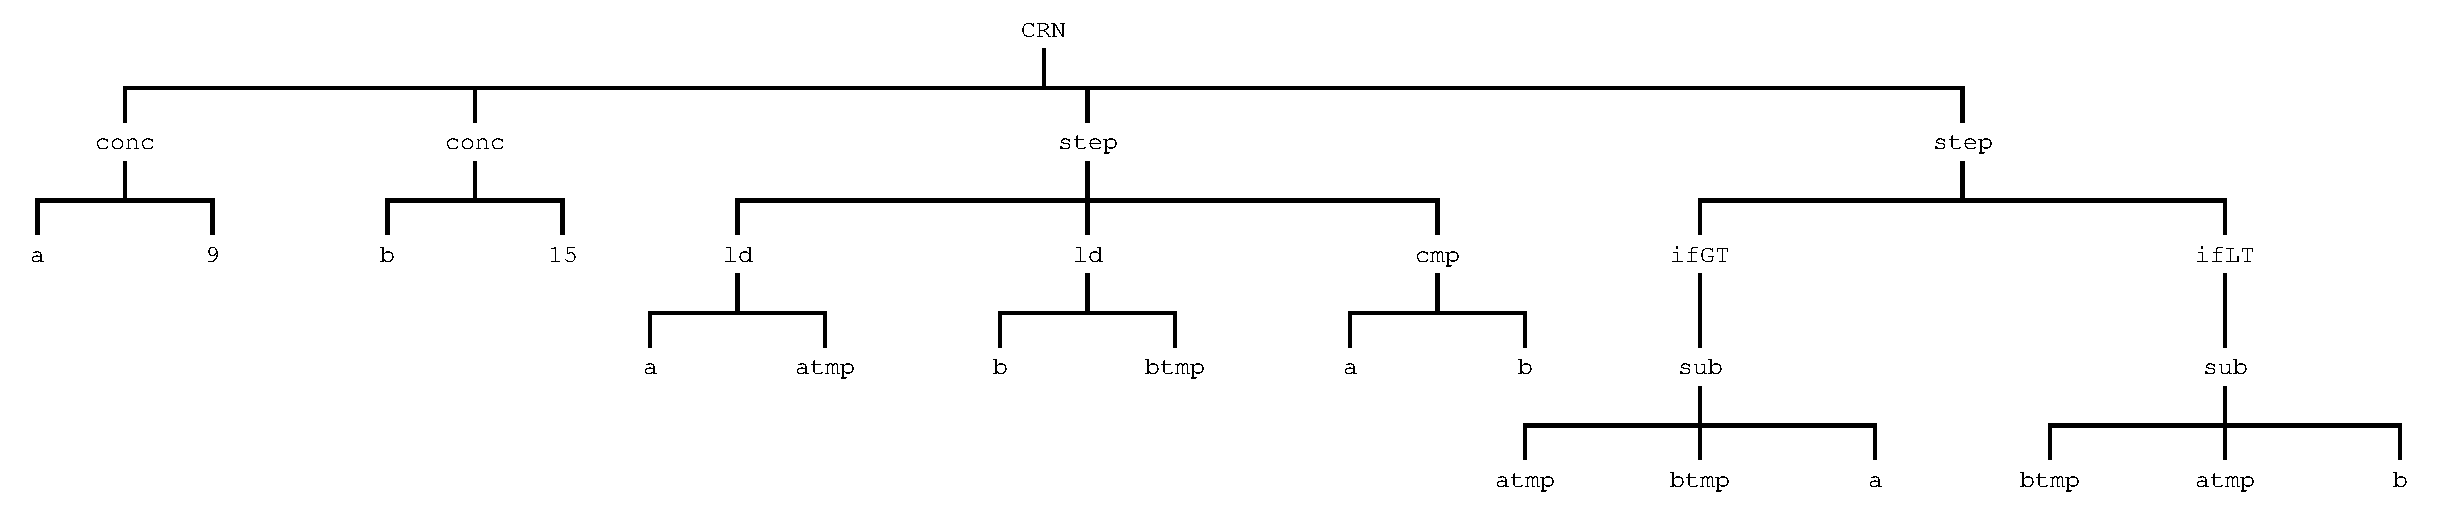
\includegraphics[width=\textwidth]{Figures/gcd-tree.pdf}
    \caption{AST of the \texttt{gcd} sample program visualized as a \textit{Drawing Tree}.}
    \label{fig:ast}
\end{figure}
The model also comprises F\# type declarations of the main syntactic categories used to construct CRN++ programs. These are displayed in Listing \ref{lst:crn-types} of the Appendix.

\subsection{Parser for CRN++} % Tjark
% Parsed string property

A parser for the CRN++ language was constructed using parser combinators of the \texttt{FParsec} library. The parser consists of a hierarchy of sub-parsers starting with parsers for all terminals such as for the \texttt{Species} type.

To avoid code repetition, helper parsers were introduced to parse pairs, triplets and lists of values with a given start, end and separator symbol. For the list parser, the grammar shown in grammar \ref{lst:listGrammar} in the appendix was used. This parser primitive could then be applied for instance to parse conditional blocks using \texttt{pListBlock "ifLE[{" "," "}]" pComputation IfLE} where \texttt{pComputation} is the parser for computations and \texttt{IfLE} is a constructor for the \texttt{Conditional} type. 

The parsers can be further combined making it easy to parse expressions such as for instance reactions using \texttt{pTriplet "rxn[" "," "]" (pList "+" pSpecies, pList "+" pSpecies, pFloat) Rxn} where \texttt{pTriplet} takes the delimiters, one parser for each element and a constructor accepting a triplet as arguments.

The full parser for the CRN++ language was implemented using these helper parsers and by letting each parser for a non-terminal rely recursively on parsers for its symbols until a terminal symbol is reached. The functionality of the parser was verified using the property that the AST of a well-formed CRN converted to plain text results in the original AST again when parsed. 


\subsection{Type Checker for CRN++} % Steffan
In order to evaluate the \hyperref[sec:well-formed]{\textit{well-formed} properties} on the generated CRN programs we had to translate these into boolean predicates in F\#. To this end, the \texttt{CrnTypeChecker} module defines 5 predicates to check each property:
\begin{enumerate}
    \item \hyperref[prop:initCmp]{\texttt{cmpBeforeConditionals}}
    \item \hyperref[prop:singleCmp]{\texttt{singleCmpForAllSteps}}
    \item \hyperref[prop:noLoadUse]{\texttt{noLoadUseProp}}
    \item \hyperref[prop:notSameIO]{\texttt{validArgsProp}}
    \item \hyperref[prop:singleAssign]{\texttt{singleAssignmentForAllSteps}}
\end{enumerate}
Another function, \texttt{isWellFormedCrn}, aggregates these results by returning the conjunction of all 5 predicates on an input CRN. 

\subsection{CRN Generator} % Tjark
% Define custom generator for FsCheck that produces well-formed CRNs
In order to use property based testing for the developed functions operating on CRNs, a generator for well-formed CRNs is needed. This task proves itself difficult, since most of the restrictions defining a well-formed CRN limit at the level of a step or even a sequence of steps, but generators usually make local choices for values. An example for this is that a species can only be the output of one active module per step. Generating a sequence of \texttt{Command}s which fulfill this limitation would require the generators for each \texttt{Command} to communicate their output species choices in order to avoid collisions. 

Although this is feasible, we chose a way of generating well-formed CRNs which involves filtering based on predicates instead. This is less efficient, since multiple attempts may be needed before all predicates are met but allows for a simpler generator implementation. The filtering is done using \texttt{Gen.where}. We further restricted the generator to not produce any reactions, since these cannot be handled by the interpreter.

To begin with, a list of initial concentrations for randomly generated species is created with a length depending on the size parameter to the generator. In general, modules are created in such a way, that the input and output species are always different. On the command level, property \ref{prop:notSameIO} is used to filter out modules which violate argument restrictions. On the step level, it is verified that the command sequence contained in the step does not violate property \ref{prop:singleCmp}, \ref{prop:noLoadUse} and \ref{prop:singleAssign}. Finally, on the level of the whole CRN it is checked that the comparison flags are initialized before use in order to satisfy property \ref{prop:initCmp}.

\subsection{CRN States}\label{sec:states} % Tjark
% Representation of step outputs from chemical reactions
In order to capture the concentrations of all molecules in an CRN throughout time, a state type is required. The state consists of a map from species to concentrations, a cycle number. Since the flag molecules are not treated as molecules with concentrations in the interpreter, two additional boolean values are contained in the state to capture the result of the latest \texttt{cmp} operation. The first boolean signalizes equality while the second signalizes whether a was greater than b. 

\subsection{Visualization} % Steffan
% Plot the sequence of generated states
% Plotly.NET
By only looking at discrete concentrations from the sequence of output states, it is difficult to determine the dynamics of the system, including judging whether a steady-state has been reached. Therefore, we used \texttt{Plotly.NET} \cite{plotly} to plot the time series of species concentrations from a finite sequence of states. Using the library allowed us to visually observe the development of the species' concentrations and how they affected each other, as demonstrated by Figure \ref{fig:counter-plot}. In addition, it was possible to focus in on certain species by toggling their visibility in the control window. 

One downside we experienced with the \texttt{Plotly.NET} library was the slow rendering of plots with long simulation times and/or multiple species. However, this was to be expected when visualizing an exponential number of data points.

\begin{figure}[h]
    \centering
    \hspace{3em}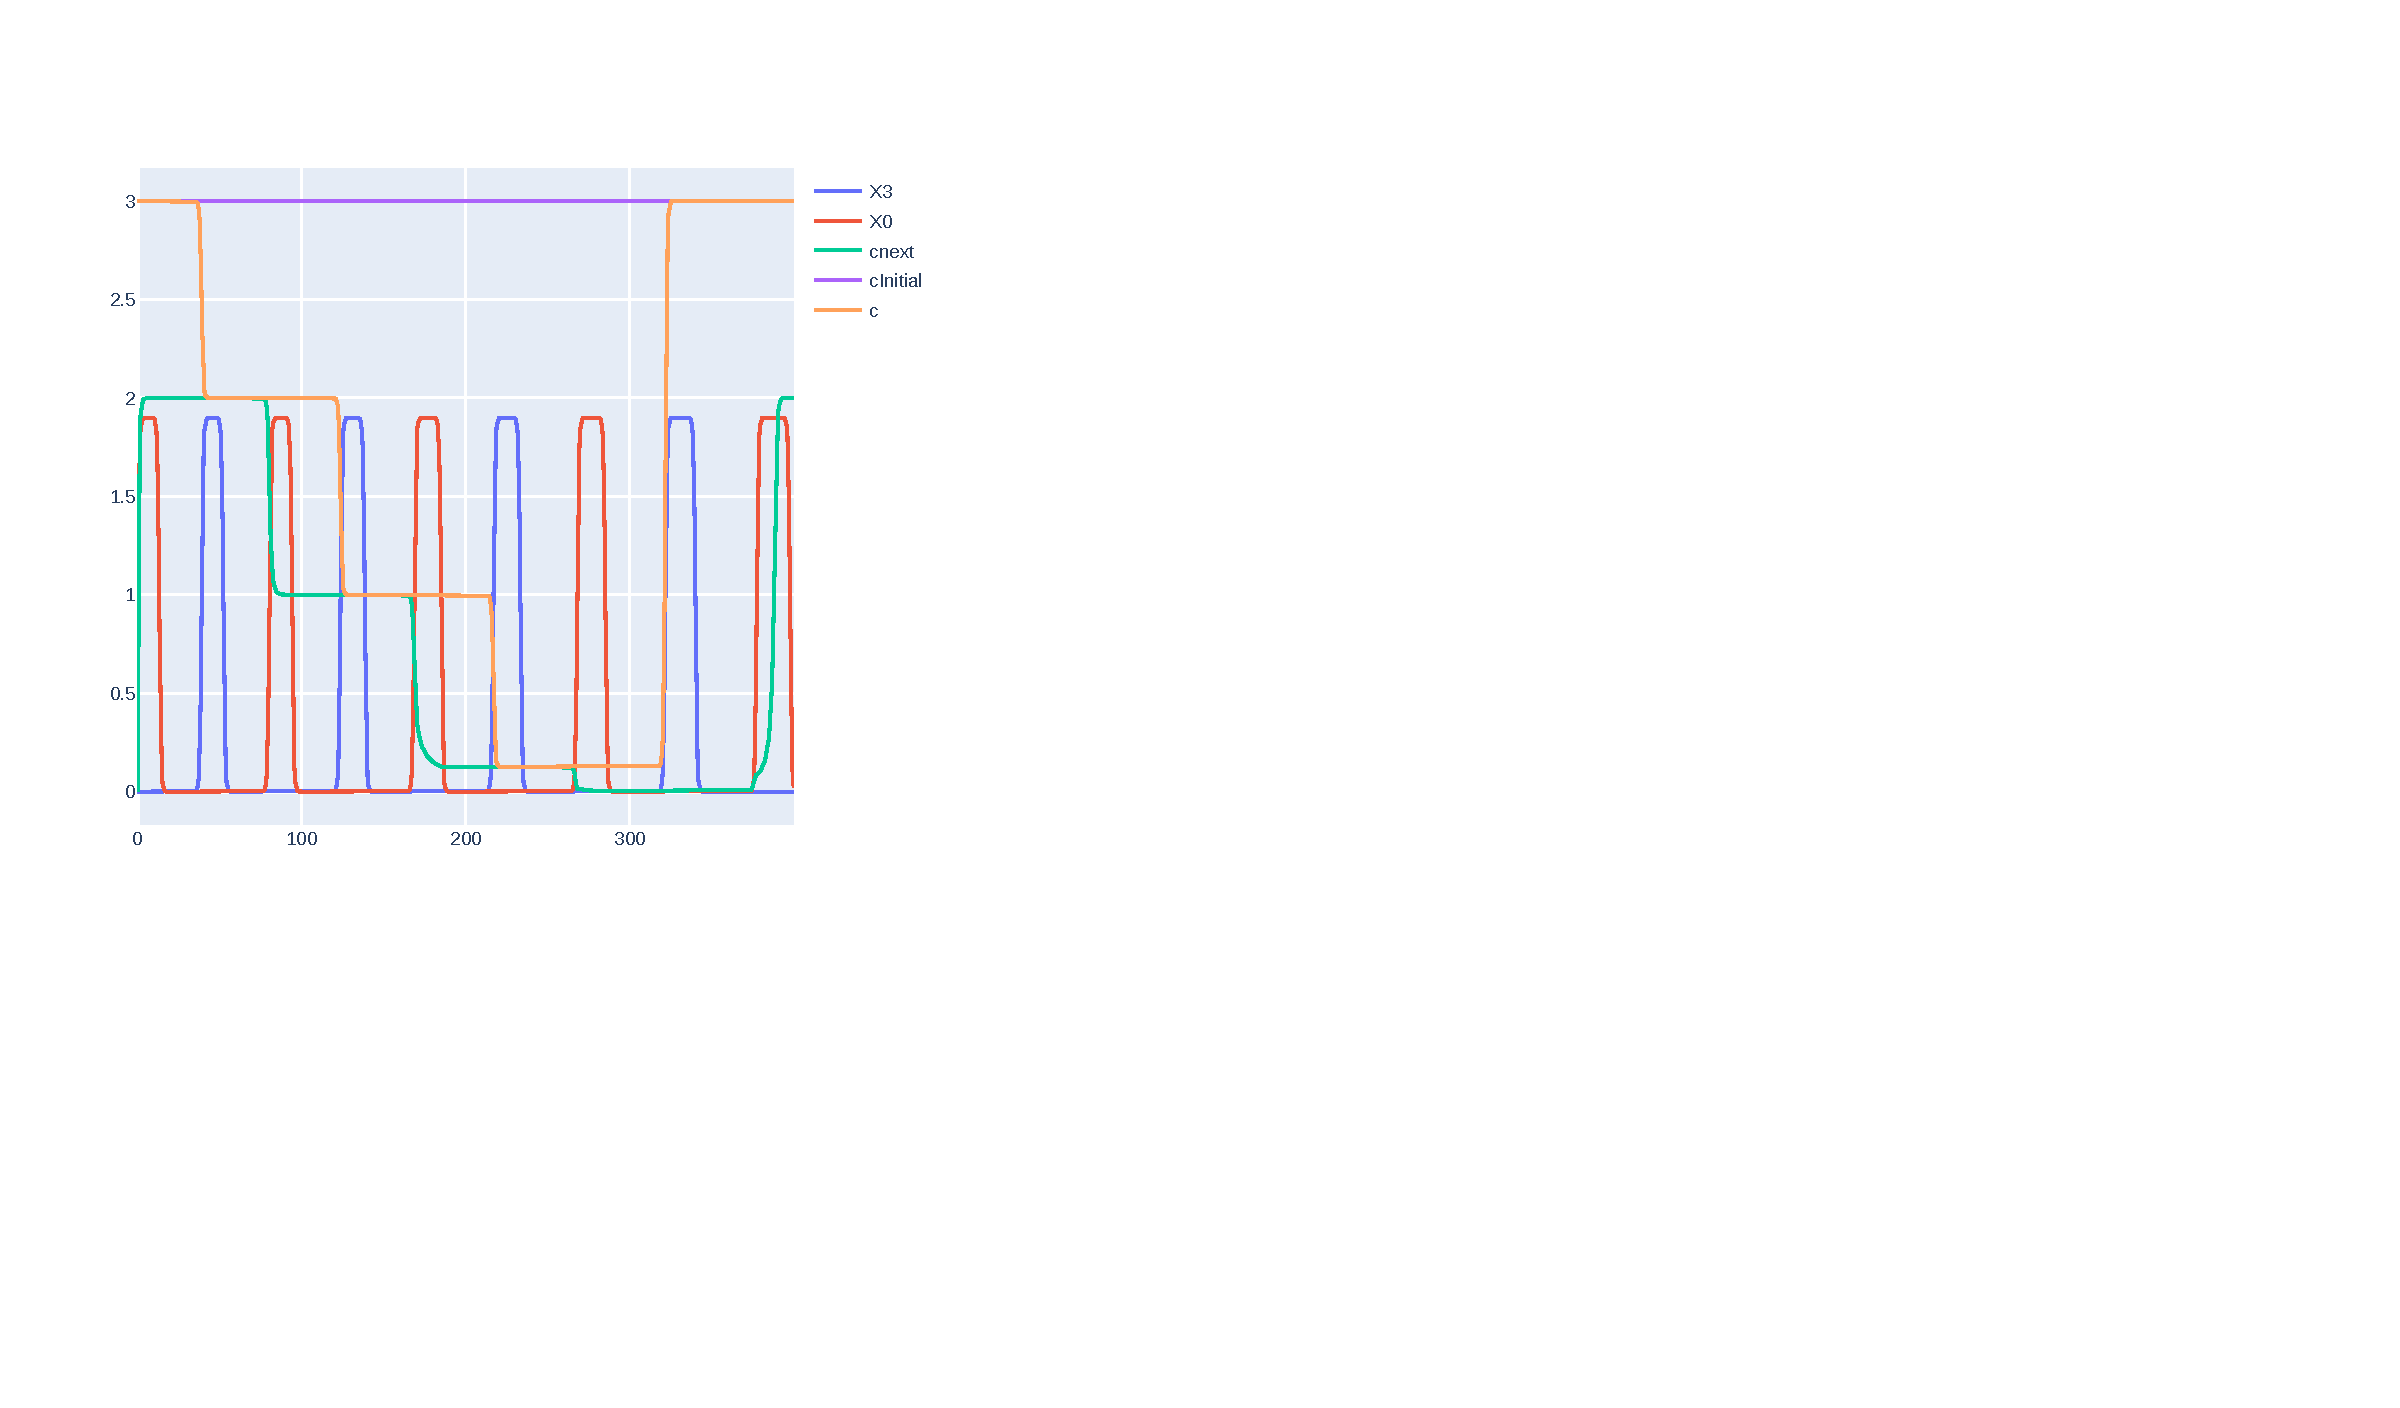
\includegraphics[width=.7\textwidth]{Figures/counter-plot.pdf}
    \caption{Species concentration of \texttt{counter} CRN++ program plotted with \texttt{Plotly.NET}.}
    \label{fig:counter-plot}
\end{figure}
